\documentclass[a4paper,12pt]{article}

%Class
	%\documentclass[a4paper,12pt]{article}

%Packages
	\usepackage{amsmath}					% Standard maths
	\usepackage{amssymb}					% Standard maths
	\usepackage{amsthm}						% Standard maths
	\usepackage{thmtools, thm-restate}% Theorem styles
	\usepackage{mathtools}
	\usepackage[newzealand]{babel}% Date/time in British format (yes, I know it says NZ)
	\usepackage{datetime}					% Date/time
	\usepackage{multirow}					% For stacked subscripts
	\usepackage{xcolor}						% For colour!
	\usepackage[normalem]{ulem}		% For strikeout
	\usepackage{isomath}
	\usepackage{fancyhdr}					% For the headers
	\usepackage{mfirstuc}					% For the headers
	\usepackage[hmargin=1in,top=0.8in,bottom=1in]{geometry} % Page margins more reasonable
	\usepackage{graphicx}					% For including graphics
	%\usepackage{float}						% For something
	\usepackage{enumitem}					% For numbering tweaks
	\usepackage{pgfplots}
	\usepackage[margin=15pt,font={footnotesize},labelfont=bf,format=hang]{caption}
\usepackage[margin=15pt,font={footnotesize},labelfont=bf,format=hang]{subcaption}
	\usepackage{url}
	\usepackage[hidelinks]{hyperref}	% For hyperlinks
	\usepackage{breakurl}
	\usepackage{cleveref}
	\usepackage[scaled=.92]{helvet}
	\newbool{show_question}
	\newbool{show_solution}
	\newcommand{\solutioninheading}{\ifbool{show_solution}{: SOLUTIONS}{}}
	\usepackage{pgfplots}
\newcommand{\ep}{\varepsilon}

\makeatletter 
\newcommand\mynobreakpar{\par\nobreak\@afterheading} 
\makeatother

    \newcommand{\question}[3]{
    	\item \textbf{#1} \mynobreakpar \nobreak \medskip % Title
    	%
    	\ifbool{show_question}{\nobreak#2}{} % Question
    	%
    	%
    	\ifbool{show_question}{\ifbool{show_solution}{\par\medskip\textbf{Solution:}}{}}{} % Both
    	\ifbool{show_solution}{#3}{} % Answer
    }			

%MATHEMATICAL SHORTCUTS
%Two and three-part definitions
	\newcommand{\twopartdef}[4]
	{	\left\{
			\begin{array}{ll}
				#1 & \mbox{if } #2 \\
				#3 & \mbox{if } #4
			\end{array}
		\right.}
%	\newcommand{\threepartdef}[6]
%	{	\left\{
%			\begin{array}{ll}
%				#1 & \mbox{if } #2 \\
%				#3 & \mbox{if } #4 \\
%				#5 & \mbox{if } #6
%			\end{array}
%		\right.}
%Blackboard bold	
	\newcommand{\N}{{\mathbb N}} 
	\newcommand{\R}{{\mathbb R}} 
	\newcommand{\C}{{\mathbb C}} 
	%Curly letters
%	\newcommand{\E}{{\mathcal E}}	
%	\newcommand{\F}{{\mathcal F}} 
%	\newcommand{\Null}{{\mathcal N}} 
%	\newcommand{\R}{\mathcal{R}} 
%	\newcommand{\Z}{\mathcal{Z}} 
%Uprights
	\newcommand{\D}{{\mathrm D}}
	\renewcommand{\d}{{\mathrm d}}
%Easy Greeks
%	\def\a{\alpha}
%	\def\g{\gamma}
%	\newcommand{\e}{{\varepsilon}}
%	\newcommand{\la}{{\lambda}}  
%	\newcommand{\om}{{\Omega}}
	\renewcommand{\epsilon}{\varepsilon}
	
%Vector operators
	\def \p {\partial}
	\newcommand{\del}{{\nabla}}
	\newcommand{\grad}{{\nabla}}
    \newcommand{\vdel}{\boldsymbol{\nabla}}
    \newcommand{\vgrad}{\boldsymbol{\nabla}}
    \newcommand{\vnabla}{\boldsymbol{\nabla}}
	\newcommand{\cross}{{\times}}
	\newcommand{\Lap}{{\nabla^2}} 
%Arrows
%	\newcommand{\goesto}[1]{\xrightarrow[#1]{}}
%hats
%	\newcommand{\nhat}{\widehat{\v{n}}}
%	\newcommand{\shat}{\widehat{\v{s}}}
	\renewcommand{\hat}{\widehat}
%Note to self
%	\newcommand{\note}[1]{[\textbf{\textsl{\MakeUppercase{#1}}}]}
	
%Stress tensor
%	\newcommand{\T}{\vg{\sigma}}

% Vectors, quaternions etc.
\renewcommand{\v}[1]{\mathbfit{#1}}      % Generic vector
\newcommand{\vc}[1]{\bm{\mathcal{#1}}}      % vector mathcal
\newcommand{\uv}[1]{\widehat{\mathbfit{#1}}}      % Generic unit vector
\newcommand{\q}[1]{\mathsfbfit{#1}}        % Generic quaternion
\renewcommand{\t}[1]{\mathsfbfit{#1}}	 % Generic tensor
\newcommand{\m}[1]{\mathsfbfit{#1}}	 % Generic matrix
\newcommand{\vu}[1]{\mathbf{#1}}         % Upright vector (for zero vector)
\newcommand{\qu}[1]{\mathbf{#1}}       % Upright quaternion (for zero quaternion)
\newcommand{\tu}[1]{\bm{\mathsf{#1}}}	 % Upright tensor (for zero tensor)

%Real and imaginary
\renewcommand{\Re}{\operatorname{Re}}
\renewcommand{\Im}{\operatorname{Im}}
	
%Non-dim numbers
%	\renewcommand{\Re}{\operatorname{Re}}
%	\newcommand{\Bi}{\operatorname{Bi}}
%	\newcommand{\Fo}{\operatorname{Fo}}
	
%Misc
\DeclareMathSymbol{\Delta}{\mathalpha}{operators}{1} % Keeps Delta upright
\DeclareMathSymbol{\Gamma}{\mathalpha}{operators}{0} % Keeps Gamma upright
	\newcommand{\cosec}{\operatorname{cosec}}
	\newcommand{\cosech}{\operatorname{cosech}}
	\newcommand{\sech}{\operatorname{sech}}
	\newcommand{\tr}{\operatorname{tr}}
	\newcommand{\erf}{\operatorname{erf}}
	\newcommand{\order}{\mathcal{O}}
%	\newcommand{\V}{\mathcal{V}} % 	CurlyV = (Bi V) / (1 + Bi)

% Differentiating 
\newcommand{\fd}[2]{\mathchoice{\frac{\d #1}{\d #2}}{\d #1/\d #2}{\d #1/\d #2}{\d #1/\d #2}}
\newcommand{\fdd}[2]{\mathchoice{\frac{\d^2 #1}{\d #2^2}}{\d^2 #1/\d #2^2}{\d^2 #1/\d #2^2}{\d^2 #1/\d #2^2}}
\newcommand{\fddd}[2]{\mathchoice{\frac{\d^3 #1}{\d #2^3}}{\d^3 #1/\d #2^3}{\d^3 #1/\d #2^3}{\d^3 #1/\d #2^3}}
\newcommand{\fdddd}[2]{\mathchoice{\frac{\d^4 #1}{\d #2^4}}{\d^4 #1/\d #2^4}{\d^4 #1/\d #2^4}{\d^4 #1/\d #2^4}}
\newcommand{\fdn}[3]{\mathchoice{\frac{\d^{#1} #2}{\d #3^{#1}}}{\d^{#1} #2/\d #3^{#1}}{\d^{#1} #2/\d #3^{#1}}{\d^{#1} #2/\d #3^{#1}}}
\newcommand{\pd}[2]{\mathchoice{\frac{\p #1}{\p #2}}{\p #1/\p #2}{\p #1/\p #2}{\p #1/\p #2}}
\newcommand{\pdd}[2]{\mathchoice{\frac{\p^2 #1}{\p #2^2}}{\p^2 #1/\p #2^2}{\p^2 #1/\p #2^2}{\p^2 #1/\p #2^2}}
\newcommand{\pddmixed}[3]{\frac{\p^2 #1}{\p #2 \p #3}}
\newcommand{\pddd}[2]{\frac{\p^3 #1}{\p #2^3}}
\newcommand{\pdn}[3]{\mathchoice{\frac{\p^{#1} #2}{\p #3^{#1}}}{\p^{#1} #2/\p #3^{#1}}{\p^{#1} #2/\p #3^{#1}}{\p^{#1} #2/\p #3^{#1}}}
	
	% Misc
\newcommand{\e}{\mathrm{e}}
\renewcommand{\i}{\mathrm{i}}
\newcommand{\dx}{\,\mathrm{d}x}
\newcommand{\dy}{\,\mathrm{d}y}
\renewcommand{\epsilon}{\varepsilon}
\renewcommand{\Re}{\operatorname{Re}}
\newcommand{\Four}{\mathcal{F}}

\newcommand{\mat}[4]{\begin{pmatrix}#1 & #2 \\ #3 & #4 \end{pmatrix}}

	%Column vectors
	\makeatletter
\newcommand\rcvector[2][\\]{\ensuremath{%
  \global\def\rc@delim{#1}%
    \negthinspace\begin{pmatrix}
      \rc@vector #2,\relax\noexpand\@eolst%
    \end{pmatrix}}}
\def\rc@vector #1,#2\@eolst{%
  \ifx\relax#2\relax
    #1
  \else
    #1\rc@delim
    \rc@vector #2\@eolst%
  \fi}
\makeatother

\newcommand{\colvec}{\rcvector}
\newcommand{\rowvec}{\rcvector}
\renewcommand{\binom}{\rcvector}
	
	%Colours
%	\newcommand{\orange}[1]{{\color{orange} #1 }}
%	\newcommand{\blue}[1]{{\color{blue} #1 }}

%Theorem styles
%	\declaretheoremstyle[headpunct={\:\:\:}, shaded={bgcolor={rgb}{0.9,0.9,0.9}, margin=5pt}]{problem}
%	\declaretheoremstyle[headpunct={\:\:\:}, shaded={rulecolor=black, rulewidth=0.4pt, bgcolor={rgb}{1,1,1}, margin=5pt}]{definition}
%	\declaretheoremstyle[headpunct={\:\:\:}, spaceabove=15pt, notefont=\bf, notebraces={(}{)}]{theorem}
%	\declaretheoremstyle[headpunct={\:\:\:}, numbered=no, spaceabove=15pt, qed={\checkmark}]{solution}
%	
%	\declaretheorem[style=definition,numberwithin=section]{definition}
%	\declaretheorem[numberlike=definition, style=theorem]{theorem}
%	\declaretheorem[numberlike=definition, style=theorem]{lemma}
%	\declaretheorem[numberlike=definition,style=problem]{problem}
%	\declaretheorem[numberlike=definition, style=theorem]{proposition}
%	\declaretheorem[numberlike=definition, style=theorem]{corollary}
%	\declaretheorem[numberlike=definition, style=theorem]{remark}
%	\declaretheorem[numberlike=definition, style=theorem]{example}
%	\declaretheorem[numberlike=definition, style=theorem]{notation}
%	\declaretheorem[style=solution]{solution}

%Depth of display breaks to allow	
	\allowdisplaybreaks[1]

%How deep do we want the Table of Contents to go?	
%	\setcounter{tocdepth}{1}

%Sections
\makeatletter
\renewcommand{\section}{\@startsection
{section}%                   % the name
{1}%                         % the level
{0mm}%                       % the indent
{-\baselineskip}%            % the before skip
{0.5\baselineskip}%          % the after skip
{\normalfont\bfseries}} % the style
\makeatother

% Wavy underline
\makeatletter
\font\sixly=lasyb10 scaled 1200
\def\tinners{\bgroup \markoverwith{\lower8.5\p@\hbox{\sixly \char58}}\ULon}
\makeatother
\newcommand{\answer}[1]{\tinners{\; #1 \;}}

%Setting the footnotes to use *,**,+ etc rather than 1,2,3	
\renewcommand{\thefootnote}{\fnsymbol{footnote}}

%Italic quote environment
%\newenvironment{quoteitalic}{\begin{quote}\itshape}{\end{quote}}

%Heading
\newcommand{\heading}[2]{
\setlength{\parindent}{0pt}
\textbf{MATH3171 (Mathematical Biology III)}

\textbf{YEAR 2025--26, \MakeUppercase{#1} TERM}
\setlength{\parskip}{3ex}

\textbf{\MakeUppercase{#2}}
%
\setlength{\parskip}{2ex}

}

%========================================================================================================================
%DOCUMENT BEGINS HERE!

\begin{document} 
%
\heading{Epiphany}{Problems class 7}
%\newcommand{\sol}[1]{}
\newcommand{\sol}[1]{\\ \hrule\hfill \\ \textcolor{blue}{\textbf{SOLUTION:}} #1 \\ \hrule\hfill}

\section*{Turing analysis of the Gierer--Meinhardt model}
    We now explore a classical model first proposed by Alfred Gierer and Hans Meinhardt to describe the branching periodic structure of the tentacles on the `head' of \emph{Hydra}, which is a genus of small freshwater organisms.  \emph{Hydra} is a fascinating organism because if you cut it in half, the `foot' will grow a new `head,' and vice-versa, so that it has the ability to regenerate completely new selves. The number and arrangement of the tentacles on the new head will be similar to the original one, but there can be some variation. See Figure \ref{hydra} for an image.\footnote{Additional fun facts: \emph{Hydra} is a fascinating organism as it does not really experience aging or natural death. They tend to be between 1mm up to 20mm in length, and have 50,000-100,000 or so cells. In comparison, humans have (very approximately) 37,200,000,000,000 cells.}
    
    We can hypothesize that the periodic arrangement of these tentacles comes from the reaction and diffusion of two signalling molecules, whose concentrations are given by $a$ and $h$ respectively. In one spatial dimension, the Gierer--Meinhardt model takes the form,
    \begin{equation}\label{a_eq}
    \pd{a}{\tau} = \beta+\rho \frac{a^2}{h} - \mu_a a + D_a \pdd{a}{x}, 
    \end{equation}
    \begin{equation}\label{h_eq}
        \pd{h}{\tau} = \rho a^2 - \mu_h h + D_h \pdd{h}{x},
    \end{equation}
    and we will assume this has the Neumann boundary conditions,
    \begin{equation}
        \pd{a}{x}(0,\tau) = \pd{a}{x}(L,\tau) = \pd{h}{x}(0,\tau) = \pd{h}{x}(L,\tau) = 0.
    \end{equation}
    Here the terms involving $\rho$ represents production of both morphogens as a function of $a$, and the linear terms $-\mu_a$ and $-\mu_h$ represent degradation rates of these molecules, with $\tau$ a dimensional time, $D_a, D_h$ diffusion coefficients respectively, and $\beta$ a basal production of the chemical $a$ (basal meaning it does not depend on the concentration $a$). All parameters are strictly greater than zero.
    
    \begin{figure}
        \centering
        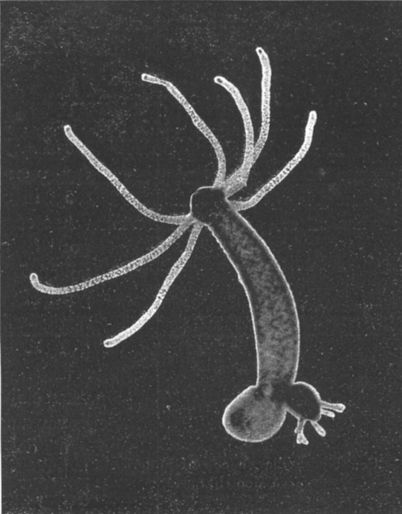
\includegraphics[width=0.28\textwidth]{Hydra-Foto}\hspace{0.1cm}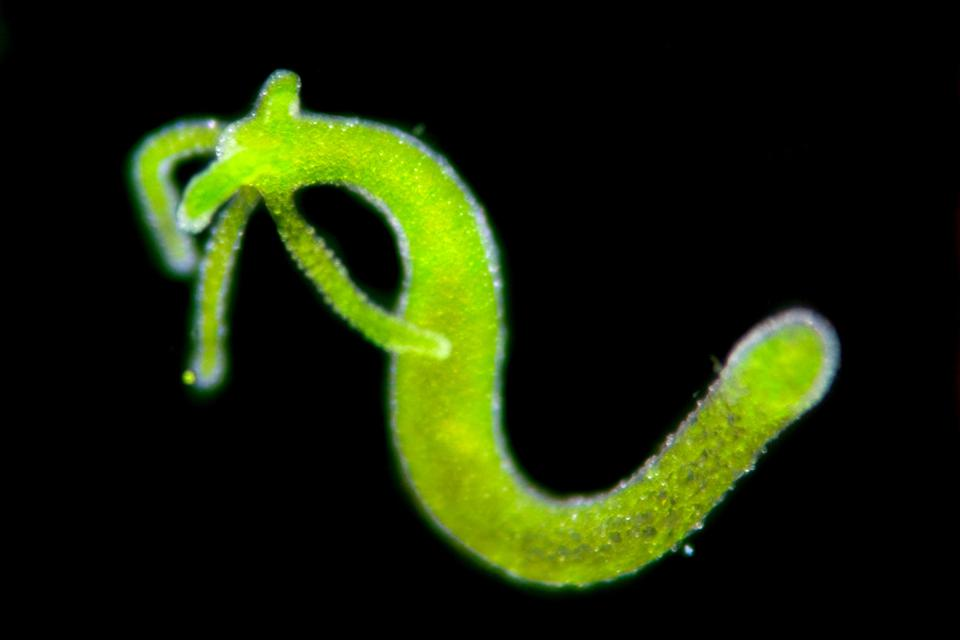
\includegraphics[width=0.54\textwidth]{hydra2}
        \caption{Images (from Wikipedia) of two different species of \emph{Hydra}. The top half or so is the `head', and the bottom half the `foot'.}
        \label{hydra}
    \end{figure}
    
    \begin{enumerate}
        \item Rescale $a = Au$, $h = Hv$, and $\tau = Tt$ to reduce the model to the non-dimensional form,
        \begin{equation}\label{u_eq}
        \pd{u}{t} = b+ \frac{u^2}{v} - c u +  \pdd{u}{x} = F(u,v)+  \pdd{u}{x}, 
        \end{equation}
        \begin{equation}\label{v_eq}
        \pd{v}{t} = u^2 - d v + D \pdd{v}{x} = G(u,v)+ D \pdd{v}{x},
        \end{equation}
        and give the expressions for $b$, $c$, $d$, and $D$ in terms of dimensional quantities. Remember you can choose $A$, $H$, and $T$ to simplify things. 
        \sol{Let $a = Au$, $h = Hv$, and $\tau = Tt$, substituting these into \eqref{a_eq}-\eqref{h_eq}, and multiplying the first equation by $T/A$ and the second by $T/H$ (so that the time derivatives have a coefficient of `$1$'), we have,
$$
    \pd{a}{t} = \frac{T \beta}{A}+\underbrace{\frac{TA\rho}{H}}_{=1} \frac{u^2}{v} - T\mu_a u + \underbrace{T D_a}_{=1} \pdd{u}{x}, 
$$
$$
        \pd{v}{t} = \underbrace{\frac{TA^2\rho}{H}}_{=1} u^2 - T\mu_h v + TD_h \pdd{v}{x}.
$$
We want the underlined coefficients of $\pdd{u}{x}$, $u^2/v$ and $u$ to all be equal to $1$, in order to match the form of the given nondimensional model. So can set up three equations in the three unknowns to find,
$$A = 1, \quad T = 1/D_a, \quad H = \frac{\rho}{D_a}.
$$ 
Finally our dimensionless\footnote{Technically, as we still have a dimensional spatial variable $x$, these constants are not quite dimensionless, but for this course that abuse of terminology is OK.} constants take the form:
$$
b = \frac{\beta}{D_a}, \quad c = \frac{\mu_a}{D_a}, \quad d = \frac{\mu_h}{D_a}, \quad D = \frac{D_h}{D_a}.
$$
}
\item Going forward, consider Equations  \eqref{u_eq}--\eqref{v_eq} with $d=1$ (to simplify the algebra a bit). Find the spatially homogeneous equilibrium solution. Write down the Jacobian of the spatially homogeneous model evaluated at this equilibrium, and hence show that the equilibrium is stable if $u_0$ satisfies,
$$
c+1>\frac{2}{u_0}, \quad \textrm{and} \quad c>0.
$$ Hint: It will be easier to work with $u_0$ as an unknown variable in the Jacobian, rather than writing it out explicitly in terms of the parameters. As $u_0$ will be proportional to $b$, it can be thought of as a proxy for this parameter.
\sol{Equilibria satisfy,
$$
b+\frac{(u_0)^2}{v_0} - c u_0 = 0, \quad (u_0)^2 - v_0 = 0.
$$
The second equation implies $v_0 = (u_0)^2$, and hence substituting this into the first equation we find $u_0 = (b+1)/c$ so $v_0 = (b+1)^2/c^2$. We can compute the Jacobian of the kinetics as:
\begin{equation*}
    \m{J}(u_0,v_0) = 
    \begin{pmatrix}
    \frac{2u_0}{v_0}-c & -\frac{(u_0)^2}{(v_0)^2}\\
    2u_0 & -1
    \end{pmatrix} = \begin{pmatrix}
    \frac{2}{u_0}-c & -\frac{1}{(u_0)^2}\\
    2u_0 & -1
    \end{pmatrix}.
\end{equation*}
The first inequality is just rearranging the requirement $\tr{\m{J}}<0$, and the second just a rearrangement of $\det{\m{J}}=c>0$.
}
\item To simplify the algebra further, assume $b = c^2-1$ so that $u_0=c$. Determine a range of values of $c$ for which this equilibrium is stable to homogeneous perturbations (that is, stable in the ODE system ignoring the diffusion terms entirely).
\sol{We have that the first inequality above (from the trace) reduces to $c^2+c>2$ and is the only nontrivial inequality for stability (as the determinant is automatically positive). We can use the quadratic formula to find the two roots or just factor this to see that we need $c(c+1)>2$, and hence $c>1$ is necessary. Since this immediately satisfies the second inequality we are done.}

\item These conditions for stability (which you have reduced to a simple requirement on $c$) satisfy the first two Turing conditions needed for a diffusion-driven instability. We will show in lecture that in order to have such an instability, the Jacobian must have a particular sign structure either of the form,
$$
\m{J} = \begin{pmatrix}
    +& +\\ -& -
\end{pmatrix}, \quad \textrm{or} \quad \m{J} = \begin{pmatrix}
    +& -\\ +& -
\end{pmatrix},
$$ and that we must have $D>1$. Use these facts to determine a second condition that $c$ must satisfy, and hence indicate which component is the activator, and which is the inhibitor. 
\sol{We have that $\m{J}$ has the sign structure,
$$
\m{J} = \begin{pmatrix}
    \frac{2}{u_0}-c & -\\
    + & -
    \end{pmatrix},
$$
and so we require that $$
\frac{2}{u_0}-c = \frac{2}{c}-c>0 \implies c < \sqrt{2},
$$
so that for stability of the equilibrium, and the correct sign structure of $\m{J}$, we require $c$ to be in the range $1 < c < \sqrt{2}$.

Hence $u$ is an activator, and $v$ is an inhibitor, so we require $D>1$.}

\item  The other two Turing conditions are given by,
$$
G_v + DF_u>0,\quad (G_v+ D F_u)^2 - 4 D (F_uG_v  -G_uF_v) >0.
$$
Write these conditions out in terms of $c$ and $D$. Using the first. determine a range that the parameter $D$ must take in order to allow for diffusion-driven instabilities, and note how this compares with the range you found in part 4 above.  Write the second condition in terms of a polynomial in $D$, and argue that for $D\gg 1$, it must be satisfied (you need not compute the exact value beyond which it is satisfied).
    \sol{The first of these can be written as,
    $$
    -1+\frac{2D}{c}-cD>0 \implies D > \frac{c}{(2-c^2)}.
    $$
    and note that this is automatically satisfied if $D>1$.
    
    The second is
    $$
    \left(-1+\frac{2D}{c}-cD\right)^2-4Dc >0.
    $$
    This second condition can be rearranged as,
    $$
    D^2 \left (c^2-4+\frac{4}{c^2} \right)-D\left (\frac{4}{c}+2c \right)+1>0. 
    $$
    There are a few ways to see what happens as $D$ increases. An easy way is to note that the coefficient of $D^2$ is zero if $c=\sqrt{2}$ (which it cannot be by assumption), and is otherwise always positive. Hence for $D \gg 1$, this quadratic term will dominate, and the inequality will always be satisfied.
    }
    \item Summarize the necessary assumptions on the various parameters for the non-dimensional model \eqref{u_eq}--\eqref{v_eq} to admit diffusion-driven instability, briefly commenting on what they mean biologically.
    \sol{Firstly we assumed that $d=1$, indicating that the timescale of inhibitor degradation $\mu_h$ was comparable to activator diffusion $D_a$. Secondly we assumed that the feed or basal production rate $b$ was equal to the square of the degradation rate $c$, that is $b=c^2$. This led to the restriction that $1 < c < \sqrt{2}$ to satisfy a stable equilibrium ($c>1$) and the correct interpretation of $u$ as an activator ($c<\sqrt{2}$). In order to use the Turing conditions, we require $L \gg 1$, and finally we have shown that for $D \gg 1$ (and in particular $D > 1>c/(1-c^2)$), we can satisfy these conditions.
    }
 \end{enumerate}


    
    
\end{document}